\chapter{TUTORIAL DO VISIUMOUSE}\label{CAP-tecnologia-visiumouse}
Neste ponto é manifestado a visão do usuário final, desde o cadastro e entrada no site para fazer o \textit{download}, até a instalação e uso do VisiUMouse. 

\section{Download do VisiUMouse}
Para qualquer usuário que deseja fazer o \textit{download} do VisiUMouse é obrigatório o cadastro, caso não tenha se cadastrado antes, caso já tenha se cadastrado em um outro momento é preciso apenas efetuar a entrada (\textit{login}), para isso foi criado uma sessão no menu que corresponde a essas funcionalidades, a 'ENTRAR', na Figura \ref{fig:site-entrar} podemos ver essa opção no canto superior direito, marcado com vermelho. Ao clicar nessa opção o usuário vai entrar na página, como mostrado em 'Página de entrada', a qual ele pode inserir seus dados para entrar no site, porém caso ele não tenha se cadastrado ele pode clicar em 'CADASTRAR', ainda na mesma página, após clicar em 'CADASTRAR' é carregado a página de cadastro, como mostrado na Figura \ref{fig:site-entrar} na 'Página de cadastro'. Para fazer o cadastro é necessário o usuário informar seus dados pessoais, se alguma informação estiver incorreta o próprio site vai indicar. 

\begin{figure}[H]
\caption{Páginas de cadastro e entrada de usuários do site.} 
\centering 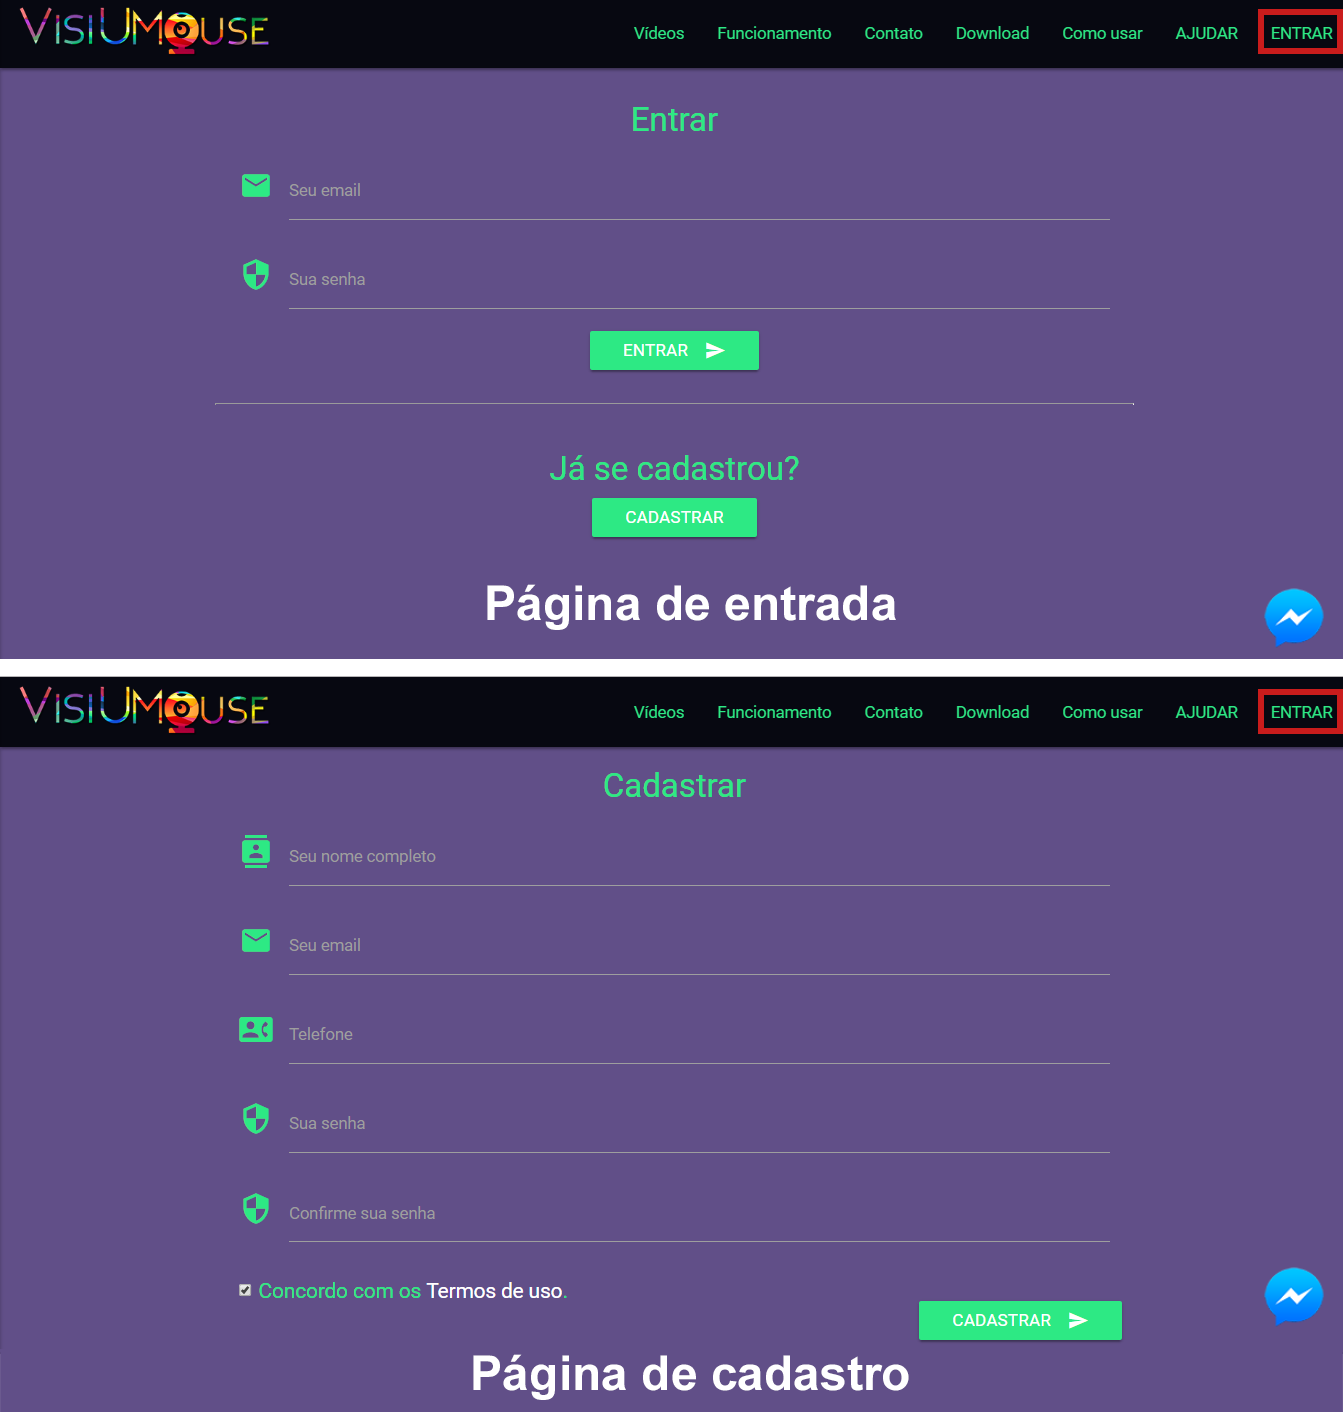
\includegraphics[scale=0.45]{img/site-entrar.png}

{\fontsize{11}{11}\selectfont \textbf{Fonte:} Elaborada pelo autor.}
\label{fig:site-entrar}
\end{figure}

Após a entrada do usuário no site é possível fazer o \textit{download} do VisiUMouse, nessa página ele pode ver uma tabela com características de cada versão, como mostrado na Figura \ref{fig:site-download}.


\section{Instalando o VisiUMouse}
A instalação do VisiUMouse segue o padrão de outros instaladores de \textit{softwares} disponíveis no mercado, a primeira tela é de apresentação, explicando o que o instalador vai fazer e se o usuário concorda; uma tela onde é configurado a pasta onde o VisiUMouse vai ser instalado; uma tela para iniciar a instalação; e, por fim, uma tela avisando que o VisiUMouse já foi instalado, como mostrado na Figura \ref{fig:visiumouse-instalador}.

\begin{figure}[H]
\caption{Telas de instalação do VisiUMouse.} 
\centering 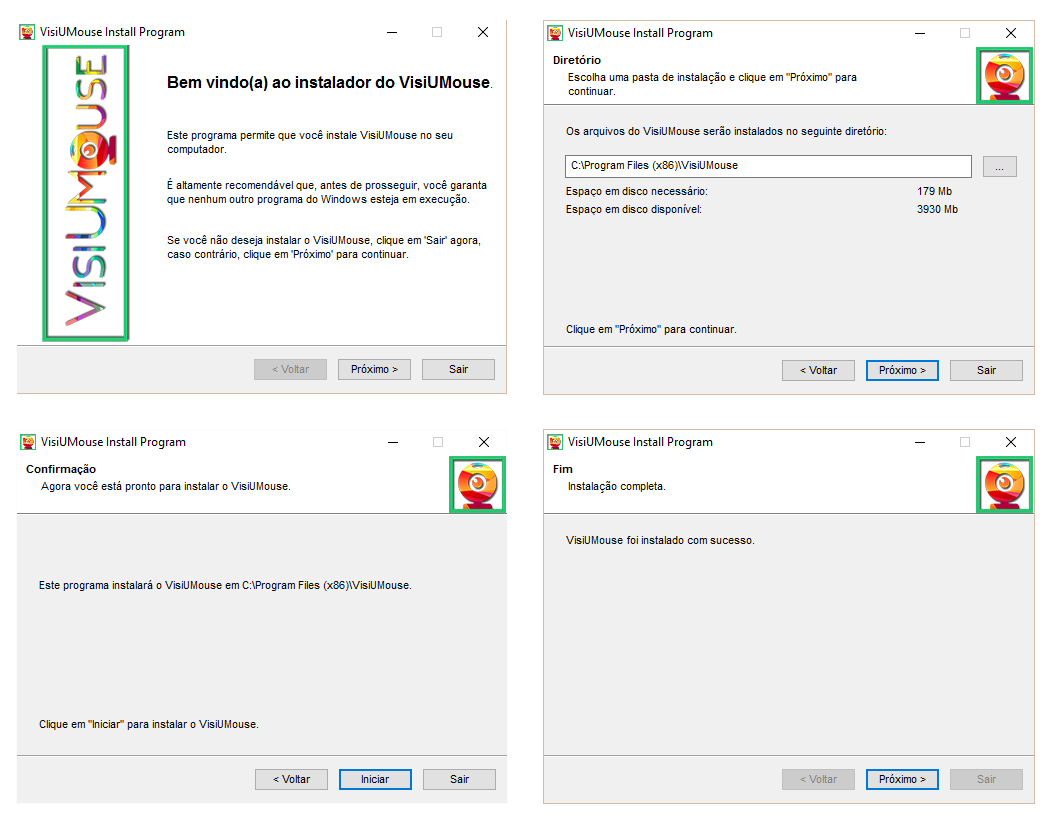
\includegraphics[scale=0.45]{img/software-instalador.png}

{\fontsize{11}{11}\selectfont \textbf{Fonte:} Elaborada pelo autor.}
\label{fig:visiumouse-instalador}
\end{figure}

\section{VisiUMouse}
Após a instalação, o VisiUMouse pode ser executado através de um atalho que foi criado na área de trabalho. A primeira tela que renderizada é a tela principal da GUI, como vista na Figura \ref{fig:visiumouse-tela-principal}, é ela que tem os primeiros passos para iniciar o controle do movimento e clique do \textit{mouse}. No primeiro momento é preciso clicar no botão 'iniciar', para iniciar a \textit{webcam}.

\begin{figure}[H]
\caption{Tela principal do VisiUMouse.} 
\centering 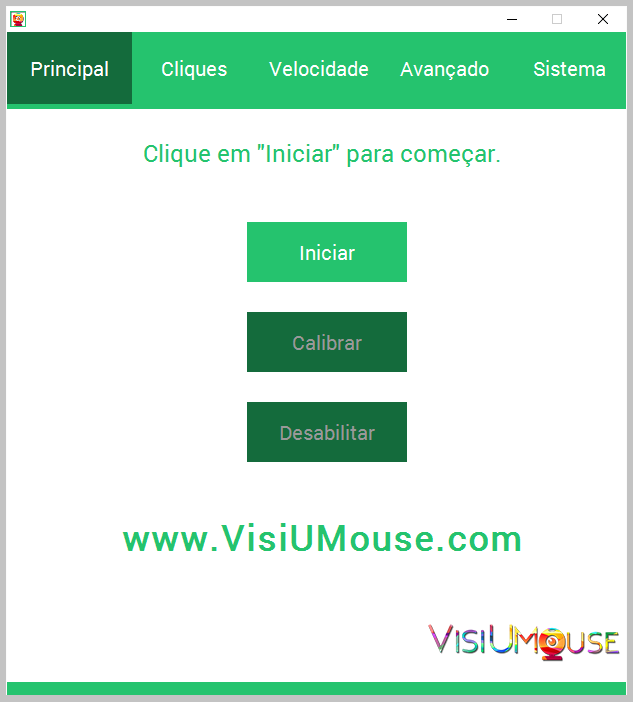
\includegraphics[scale=.5]{img/visiumouse-tela-principal-v216.png}

\textbf{Fonte:} Elaborada pelo autor.
\label{fig:visiumouse-tela-principal}
\end{figure}

A inicialização da \textit{webcam} é dada pela tela de captura de vídeo, como visto na Figura \ref{fig:visiumouse-tela-captura-video}, ela permite que e o usuário tenha o retorno se ele esta posicionado no centro da tela, e se é possível rastrear seus olhos, os retângulos vermelho em volta dos olhos mostram o rastreamento dos olhos. Nessa tela o usuário pode ver o 'MODO' da aplicação, como visto no canto superior esquerdo da Figura, podendo dar 3 avisos: 'FUNCIONAL' mostrando que já é possível controlar o movimento do \textit{mouse}; 'DESABILITADO' informa o usuário que ele não está controlando o \textit{mouse}; 'CALIBRANDO (FIQUE PARADO(A))' que informa o usuário que não deve se mover por que o VisiUMouse esta calibrando.

No segundo momento é preciso clicar em 'calibrar' para calibrar o VisiUMouse, ou seja o usuário precisa ficar parado até receber o aviso que o modo está funcional, como visto na Figura \ref{fig:visiumouse-tela-captura-video}. Após a calibração o usuário é capaz de controlar o \textit{mouse} e para desabilitar o controle basta clicar em 'desabilitar' na tela principal, como visto na Figura \ref{fig:visiumouse-tela-principal}.

\begin{figure}[H]
\caption{Tela de captura de vídeo.} 
\centering 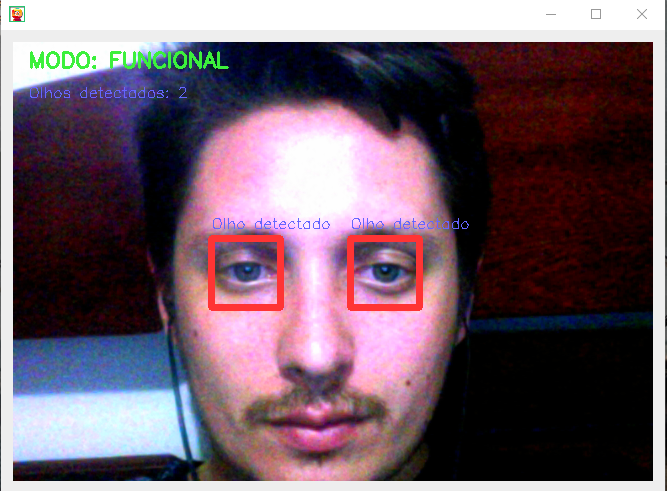
\includegraphics[scale=.45]{img/visiumouse-tela-captura-video.png}

{\fontsize{11}{11}\selectfont \textbf{Fonte:} Elaborada pelo autor.}
\label{fig:visiumouse-tela-captura-video}
\end{figure}



\chapter{DOCUMENTAÇÃO CASO DE USO}
\label{Apx:A}
\begin{longtable}{|l|l|}
\caption{Documentação Caso de Uso \textit{Iniciar aplicação}.} \label{tab:dcu-1} \\
\hline 
\multicolumn{1}{|c|}{\textbf{Nome do Caso de Uso}} & 
\multicolumn{1}{c|}{\textbf{Funcionamento do Software}} \\ \hline 
\endfirsthead
\hline
Caso de Uso Geral &  \\ \hline
Ator Principal & Usuário, responsável\\ \hline
Ator Secundário &  \\ \hline
Resumo & Usuário/responsável iniciando a aplicação. \\ \hline 
Pré-condições &  O Software deve ter sido executado. \\ \hline 
Pós-condições &  Mostrar a tela de captura de vídeo. \\ \hline
 Ações do Ator& Ações do Sistema \\ \hline
 1.	Clicar em iniciar na tela principal.&  \\ \hline
\end{longtable}

\begin{longtable}{|l|l|}
\caption{Documentação Caso de Uso \textit{Configurar}.} \label{tab:dcu-1} \\
\hline 
\multicolumn{1}{|c|}{\textbf{Nome do Caso de Uso}} & 
\multicolumn{1}{c|}{\textbf{Funcionamento do Software}} \\ \hline 
\endfirsthead
\hline
Caso de Uso Geral &  \\ \hline
Ator Principal & Usuário\\ \hline
Ator Secundário & \\ \hline
Resumo & Usuário fazendo configuração. \\ \hline 
Pré-condições &  Estar na parte de configuração. \\ \hline 
Pós-condições &  Configuração. \\ \hline
 Ações do Ator& Ações do Sistema \\ \hline
 1.	Clicar em uma das configurações.&  \\ \hline
 2.	Configurar um parâmetro.&  \\ \hline
 & 3. Envia a novo parâmetro para o sistema. \\ \hline
\end{longtable}

\begin{longtable}{|l|l|}
\caption{Documentação Caso de Uso \textit{Reconhecer olhos}.} \label{tab:dcu-1} \\
\hline 
\multicolumn{1}{|c|}{\textbf{Nome do Caso de Uso}} & 
\multicolumn{1}{c|}{\textbf{Funcionamento do Software}} \\ \hline 
\endfirsthead
\hline
Caso de Uso Geral &  \\ \hline
Ator Principal & Usuário\\ \hline
Ator Secundário & \\ \hline
Resumo & Sistema rastreando os olhos do usuário. \\ \hline 
Pré-condições &  Aplicação iniciada. \\ \hline 
Pós-condições &  Leitura da posição dos olhos. \\ \hline
 Ações do Ator& Ações do Sistema \\ \hline
 1.	Clicar em calibrar.&  \\ \hline
 & 2. Rastrear a posição dos olhos do usuário. \\ \hline
\end{longtable}

\begin{longtable}{|l|l|}
\caption{Documentação Caso de Uso \textit{Definir olhos principais}.} \label{tab:dcu-1} \\
\hline 
\multicolumn{1}{|c|}{\textbf{Nome do Caso de Uso}} & 
\multicolumn{1}{c|}{\textbf{Funcionamento do Software}} \\ \hline 
\endfirsthead
\hline
Caso de Uso Geral &  \\ \hline
Ator Principal & Usuário\\ \hline
Ator Secundário & \\ \hline
Resumo & Define os olhos do usuário. \\ \hline 
Pré-condições &  Aplicação calibrada. \\ \hline 
Pós-condições &  \\ \hline
 Ações do Ator& Ações do Sistema \\ \hline
 & 1. Identifica os olhos. \\ \hline
\end{longtable}

\begin{longtable}{|l|l|}
\caption{Documentação Caso de Uso \textit{Controlar mouse}.} \label{tab:dcu-1} \\
\hline 
\multicolumn{1}{|c|}{\textbf{Nome do Caso de Uso}} & 
\multicolumn{1}{c|}{\textbf{Funcionamento do Software}} \\ \hline 
\endfirsthead
\hline
Caso de Uso Geral &  \\ \hline
Ator Principal & Usuário\\ \hline
Ator Secundário & \\ \hline
Resumo & Controle do mouse. \\ \hline 
Pré-condições &  Olhos identificados. \\ \hline 
Pós-condições &  \\ \hline
Ações do Ator& Ações do Sistema \\ \hline
 1. Controle do mouse. &  \\ \hline
\end{longtable}


\begin{comment}
Exemplos do Template

\chapter{Exemplo do pacote Algorithm}
\label{Apx:B}

\begin{algorithm}[!h]
\caption{Estimador ML otimizado.}\label{Alg:MAXVER}
\begin{algorithmic}[1]
\STATE Inicializar o contador: $j\leftarrow 1$;%
\STATE Fixar o limiar de variação das estimativas: $e_{\mathrm{out}}\leftarrow 10^{-4}$;%
\STATE Fixar o número máximo de iterações: $N\leftarrow 1000$;%
\STATE Computar o ponto inicial: $\hat \gamma(0)$;%
\STATE Determinar o limiar inicial: $e_1 \leftarrow1000$;%
\STATE Estabelecer o valor inicial de $\alpha$: $\hat \alpha(0) \leftarrow -10^{-6}$;%
\WHILE{ $e_j \geq e_{\mathrm{out}}$ e $ j\leq M$}
    \STATE Solucionar $\hat \alpha_j\leftarrow {\arg \max}_{\alpha}\;{l_1(\alpha; \gamma_{j-1},\mathbf{z},n)}$;%
    \STATE Solucionar $\hat \gamma_j\leftarrow {\arg \max}_{\gamma}\;{l_2(\gamma; \alpha_j,\mathbf{z},n)}$;%
    \STATE $j\leftarrow j+1$
    \STATE Computar o critério de convergência: $e_j$;%
\ENDWHILE
\end{algorithmic}
\end{algorithm}
\end{comment}